%**************************************************************************************
% License:
% CC BY-NC-SA 4.0 (http://creativecommons.org/licenses/by-nc-sa/4.0/)
%**************************************************************************************

\documentclass{beamer}

\mode<presentation>{%
  \usetheme{Madrid}

  % Burnt orange
  \definecolor{burntorange}{rgb}{0.8,0.33,0.0}

  \makeatletter
    % Now @ is a letter, so this works:
    \colorlet{beamer@blendedblue}{burntorange}
    \setbeamercolor*{palette secondary}{use=structure,fg=white,bg=burntorange!80!black}
    \setbeamercolor*{palette tertiary}{use=structure,fg=white,bg=burntorange!60!black}
  \makeatother

  % Background
  \definecolor{paleyellow}{rgb}{1.0,1.0,0.953}
  \setbeamercolor{background canvas}{bg=paleyellow}
}

\usepackage{amsmath}
\usepackage{bm}
\usepackage{breqn}
\usepackage{graphicx} % for figures
\usepackage{subcaption} % for subplots 
\usepackage[labelsep=space,tableposition=top]{caption}
\renewcommand{\figurename}{Fig.} 
\usepackage{cleveref}
\usepackage{booktabs} % Allows the use of \toprule, \midrule and \bottomrule in tables
\usepackage{listings}
\usepackage{xcolor}

\usepackage{adjustbox}
\usepackage{array}


% Define a two‐argument column type R{<angle>}{<lap>}
\newcolumntype{R}[2]{%
  >{\adjustbox{angle=#1,lap=\width-(#2)}\bgroup}%
  <{\egroup}%
}

% A simple macro to rotate a single header cell by 90°,
% using a 1em “lap” so it tucks in nicely.
\newcommand*\rot[1]{%
  \multicolumn{1}{R{90}{1em}}{#1}%
}

% Code styling
\definecolor{codegreen}{rgb}{0,0.6,0}
\definecolor{codegray}{rgb}{0.5,0.5,0.5}
\definecolor{codepurple}{rgb}{0.58,0,0.82}
\definecolor{backcolour}{rgb}{0.95,0.95,0.92}

\lstdefinestyle{mystyle}{
    backgroundcolor=\color{backcolour},   
    commentstyle=\color{codegreen},
    keywordstyle=\color{magenta},
    numberstyle=\tiny\color{codegray},
    stringstyle=\color{codepurple},
    basicstyle=\ttfamily\footnotesize,
    breakatwhitespace=false,         
    breaklines=true,                 
    captionpos=b,                    
    keepspaces=true,                 
    numbers=left,                    
    numbersep=5pt,                  
    showspaces=false,                
    showstringspaces=false,
    showtabs=false,                  
    tabsize=2
}
\lstset{style=mystyle}

% To print 2 slides on a page
%\usepackage{handoutWithNotes}
%\pgfpagesuselayout{2 on 1}[border shrink=2mm]
%----------------------------------------------------------------------------------------
%   TITLE PAGE
%----------------------------------------------------------------------------------------
% The short title appears at the bottom of every slide, the full title is only on the title page
\title[CE397: Multi-Layer Perceptron]{CE397 Scientific Machine Learning: Multi-Layer Perceptron} 
\author{Krishna Kumar} % name
\institute[UT Austin] % institution 
{
University of Texas at Austin \\
\medskip
\textit{
  \url{krishnak@utexas.edu}} % Your email address
}
\date{} % Date, can be changed to a custom date

\begin{document}

\begin{frame}
\titlepage % title page as the first slide
\end{frame}

\begin{frame}
 % Table of contents slide, comment this block out to remove it
 \frametitle{Overview}
 % Throughout your presentation, if you choose to use \section{} and \subsection{} 
 % commands, these %will automatically be printed on this slide as an overview 
 \tableofcontents
\end{frame}

%----------------------------------------------------------------------------------------
% slides
%----------------------------------------------------------------------------------------

%------------------------------------------------
\section{Introduction to Multi-Layer Perceptron}
%------------------------------------------------

\subsection{From Perceptron to MLP}
%------------------------------------------------
\begin{frame}
\frametitle{The Perceptron: Basic Building Block}
\begin{figure}
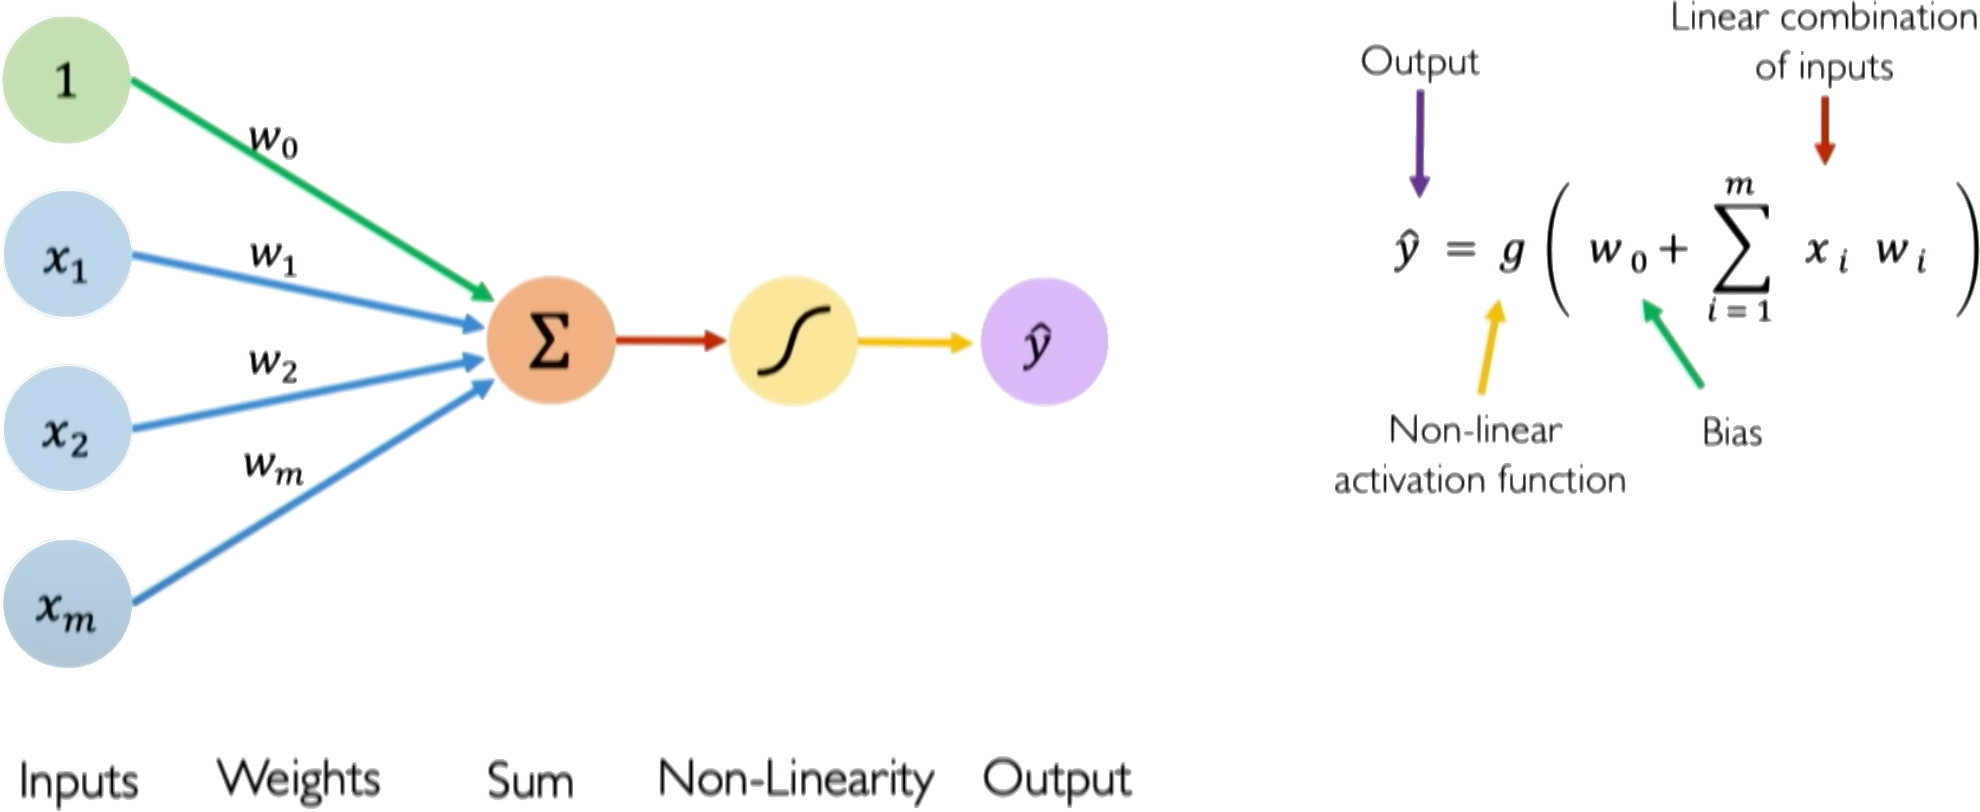
\includegraphics[width=0.7\textwidth]{perceptron.png}
\end{figure}

\begin{itemize}
    \item Single layer neural network
    \item Linear combination: $z = w_0 + \boldsymbol{w}^T\boldsymbol{x}$
    \item Activation function: $\hat{y} = g(z)$
    \item Limited to linearly separable problems
\end{itemize}
\end{frame}

%------------------------------------------------
\begin{frame}
\frametitle{Multi-Output Perceptrons}
\begin{figure}
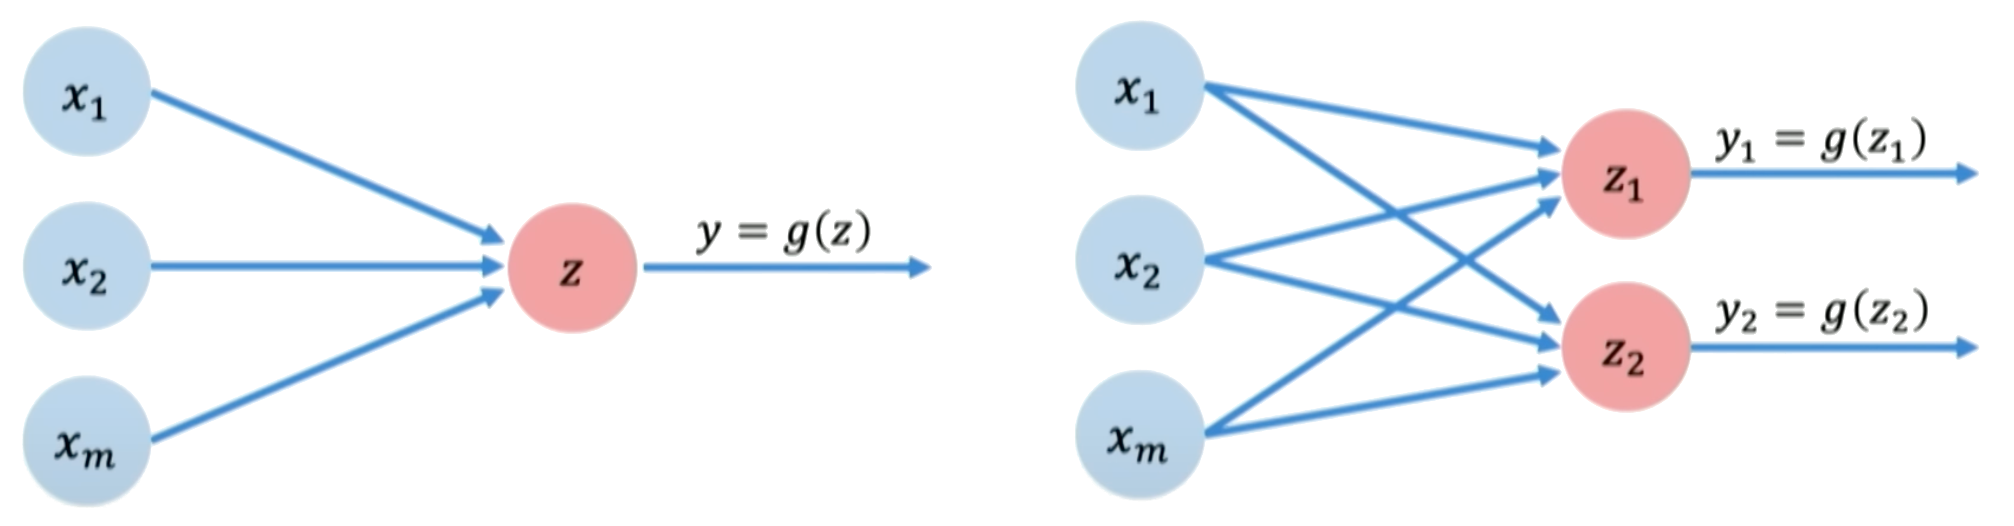
\includegraphics[width=0.8\textwidth]{multioutput-perceptrons.png}
\end{figure}

For multiple outputs, we use multiple perceptrons:
\begin{align}
z_i &= b_i + \sum_{j=1}^{m} w_{j,i} x_j \\
\hat{y}_i &= g(z_i)
\end{align}
\end{frame}

%------------------------------------------------
\begin{frame}
\frametitle{Single-Layer Neural Network}
\begin{figure}
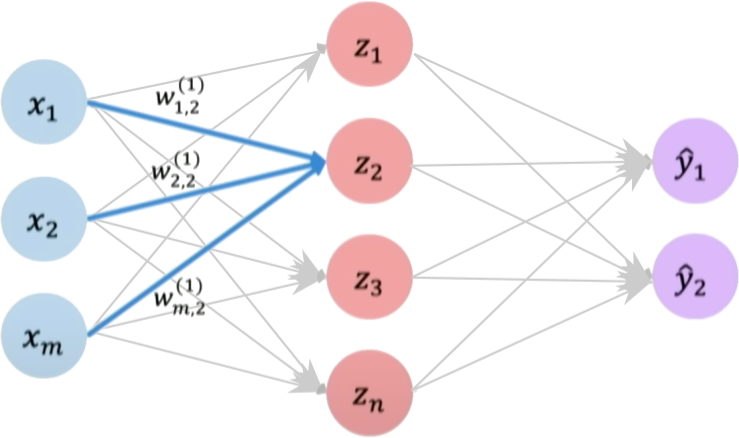
\includegraphics[width=0.8\textwidth]{single-layer-nn1.png}
\end{figure}

Dense layers: All inputs connected to all outputs
\begin{equation}
z_2 = b_2^{(1)} + \sum_{j=1}^m w_{j,2}^{(1)} x_j
\end{equation}
\end{frame}

%------------------------------------------------
\begin{frame}
\frametitle{Multi-Layer Perceptron Architecture}
\begin{figure}
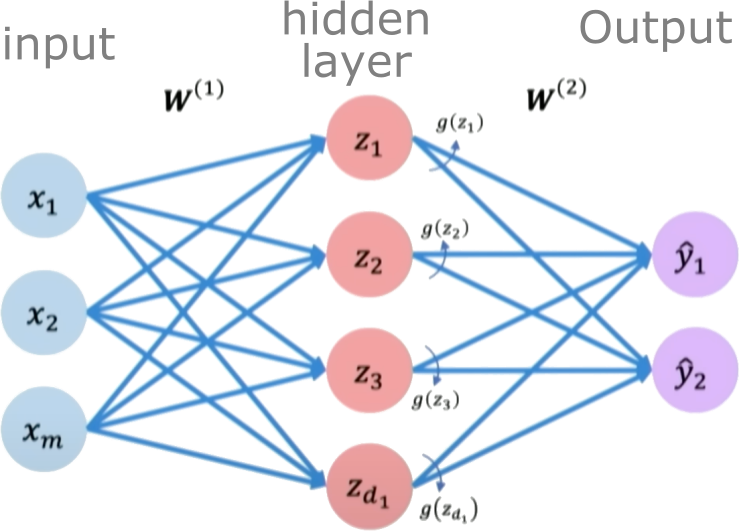
\includegraphics[width=0.8\textwidth]{single-layer-nn2.png}
\end{figure}

Hidden layers enable learning complex non-linear relationships:
\begin{align}
z_i^{(1)} &= b_i^{(1)} + \sum_{j=1}^{m} w_{j,i}^{(1)} x_j \\
\hat{y}_i &= g\left(b_i^{(2)} + \sum_{j=1}^{d_1} w_{j,i}^{(2)} g(z_j^{(1)})\right)
\end{align}
\end{frame}

%------------------------------------------------
\section{Activation Functions}
%------------------------------------------------

\subsection{Non-linear Activation Functions}
%------------------------------------------------
\begin{frame}
\frametitle{Why Non-linear Activation Functions?}
\begin{figure}
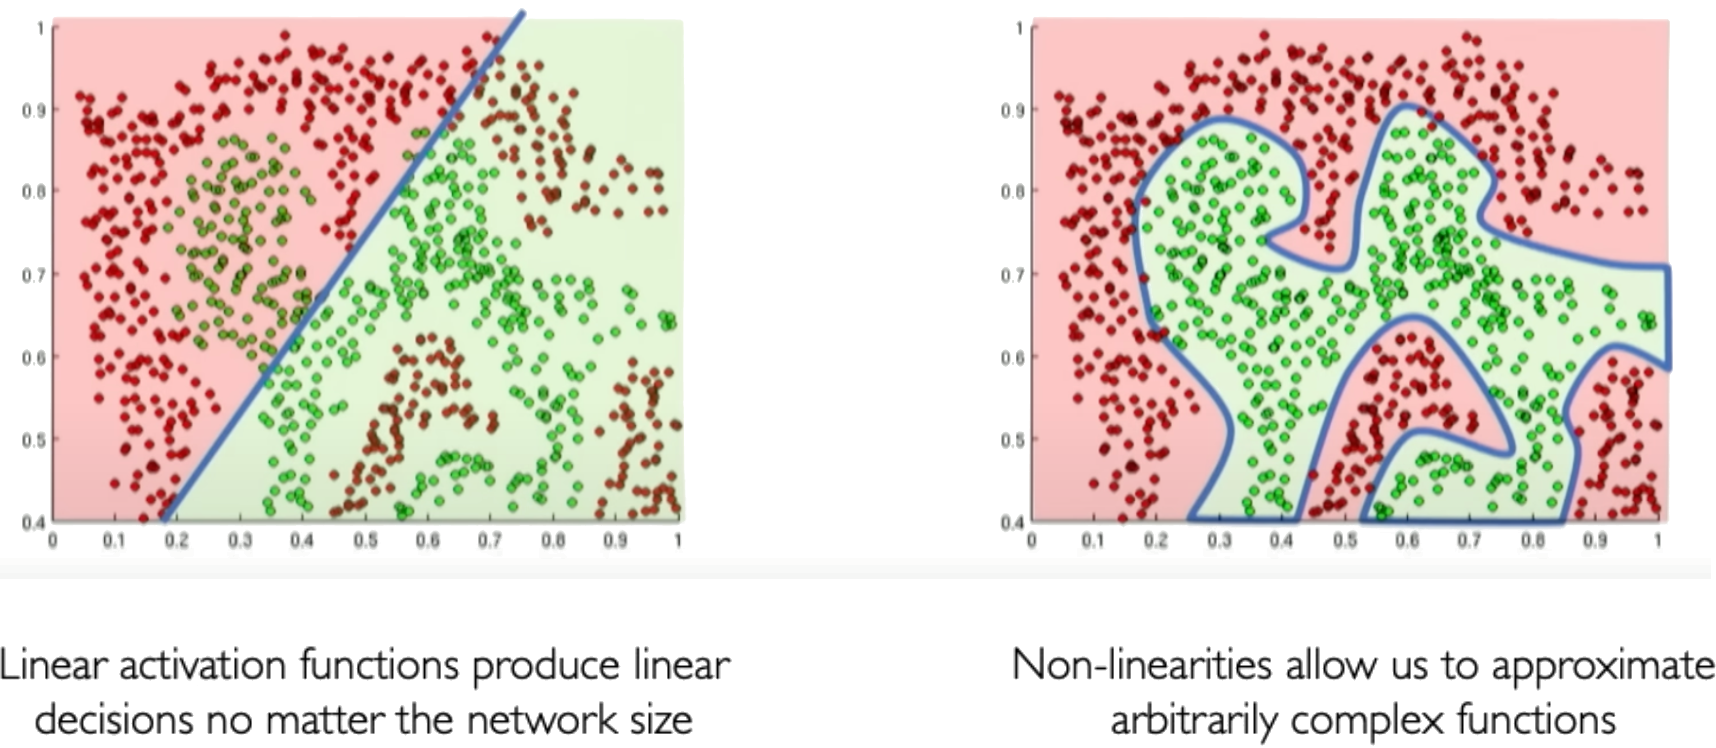
\includegraphics[width=0.8\textwidth]{why-activation.png}
\end{figure}

Without non-linear activations:
\begin{itemize}
    \item Network becomes equivalent to linear regression
    \item Cannot learn complex patterns
    \item Multiple layers provide no benefit
\end{itemize}
\end{frame}

%------------------------------------------------
\begin{frame}
\frametitle{Sigmoid Activation Function}
\begin{columns}
\begin{column}{0.5\textwidth}
Mathematical form:
\begin{equation}
\sigma(x) = \frac{1}{1 + e^{-x}}
\end{equation}

Properties:
\begin{itemize}
    \item Output range: $(0, 1)$
    \item Smooth and differentiable
    \item Saturates for large $|x|$
    \item Vanishing gradient problem
\end{itemize}
\end{column}
\begin{column}{0.5\textwidth}
Derivative:
\begin{equation}
\frac{d\sigma}{dx} = \sigma(x)(1 - \sigma(x))
\end{equation}

Applications:
\begin{itemize}
    \item Binary classification
    \item Probability outputs
    \item Historically popular
\end{itemize}
\end{column}
\end{columns}
\end{frame}

%------------------------------------------------
\begin{frame}
\frametitle{Hyperbolic Tangent (Tanh)}
\begin{columns}
\begin{column}{0.5\textwidth}
Mathematical form:
\begin{equation}
\tanh(x) = \frac{e^x - e^{-x}}{e^x + e^{-x}}
\end{equation}

Properties:
\begin{itemize}
    \item Output range: $(-1, 1)$
    \item Zero-centered
    \item Still suffers from vanishing gradients
\end{itemize}
\end{column}
\begin{column}{0.5\textwidth}
Derivative:
\begin{equation}
\frac{d\tanh}{dx} = 1 - \tanh^2(x)
\end{equation}

Advantages:
\begin{itemize}
    \item Better than sigmoid for hidden layers
    \item Symmetric around zero
    \item Faster convergence
\end{itemize}
\end{column}
\end{columns}
\end{frame}

%------------------------------------------------
\begin{frame}
\frametitle{ReLU: Rectified Linear Unit}
\begin{columns}
\begin{column}{0.5\textwidth}
Mathematical form:
\begin{equation}
\text{ReLU}(x) = \max(0, x)
\end{equation}

Properties:
\begin{itemize}
    \item Output range: $[0, \infty)$
    \item Computationally efficient
    \item Alleviates vanishing gradients
    \item "Dying ReLU" problem
\end{itemize}
\end{column}
\begin{column}{0.5\textwidth}
Derivative:
\begin{equation}
\frac{d\text{ReLU}}{dx} = \begin{cases} 
1 & \text{if } x > 0 \\
0 & \text{if } x \leq 0
\end{cases}
\end{equation}

Advantages:
\begin{itemize}
    \item Most popular activation
    \item Speeds up training
    \item Sparse activation
\end{itemize}
\end{column}
\end{columns}
\end{frame}

%------------------------------------------------
\begin{frame}
\frametitle{Leaky ReLU}
\begin{columns}
\begin{column}{0.5\textwidth}
Mathematical form:
\begin{equation}
\text{LeakyReLU}(x) = \max(\alpha x, x)
\end{equation}

where $\alpha$ is a small positive constant (e.g., 0.01)

Properties:
\begin{itemize}
    \item Solves "dying ReLU" problem
    \item Non-zero gradient for negative inputs
    \item Better gradient flow
\end{itemize}
\end{column}
\begin{column}{0.5\textwidth}
Derivative:
\begin{equation}
\frac{d\text{LeakyReLU}}{dx} = \begin{cases} 
1 & \text{if } x > 0 \\
\alpha & \text{if } x \leq 0
\end{cases}
\end{equation}

Use Cases:
\begin{itemize}
    \item General-purpose activation
    \item When ReLU neurons die
    \item Stable training
\end{itemize}
\end{column}
\end{columns}
\end{frame}

%------------------------------------------------
\section{Universal Approximation Theorem}
%------------------------------------------------

\begin{frame}
\frametitle{Universal Approximation Theorem}
\textbf{Theorem:} MLPs with:
\begin{itemize}
    \item At least one hidden layer
    \item Sufficient number of hidden units
    \item Non-linear activation functions
\end{itemize}

can approximate any continuous function on a compact subset of $\mathbb{R}^n$ to arbitrary accuracy.

\vspace{1em}

\textbf{Mathematical Statement:}
Finite sums of the form:
\begin{equation}
G(x) = \sum_{j=1}^{N} \alpha_j \phi\left(\sum_{i=1}^{n} w_{ji} x_i + \theta_j\right)
\end{equation}
are dense in $C(I_n)$ (continuous functions on unit hypercube).
\end{frame}

%------------------------------------------------
\section{Training MLPs}
%------------------------------------------------

\subsection{Loss Functions}
%------------------------------------------------
\begin{frame}
\frametitle{Loss Functions}
\textbf{Mean Squared Error (MSE)} - For regression:
\begin{align}
\mathcal{L}(\boldsymbol{w}) &= \frac{1}{2N} \sum_{i=1}^{N} |\|\boldsymbol{y}^{(i)} - \hat{\boldsymbol{y}}^{(i)}\||^2 \\
&= \frac{1}{2N} \sum_{i=1}^{N} \sum_{j=1}^{k} (y_j^{(i)} - \hat{y}_j^{(i)})^2
\end{align}

\textbf{Cross-Entropy Loss} - For classification:
\begin{align}
\mathcal{L}(\boldsymbol{w}) &= -\frac{1}{N} \sum_{i=1}^{N} \sum_{j=1}^{k} y_j^{(i)} \log(\hat{y}_j^{(i)})
\end{align}
\end{frame}

%------------------------------------------------
\subsection{Backpropagation}
%------------------------------------------------
\begin{frame}
\frametitle{Backpropagation Algorithm}
Computes gradients using the chain rule:

\textbf{Forward Pass:} Compute activations layer by layer
\begin{align}
\boldsymbol{a}^{(0)} &= \boldsymbol{x} \\
\boldsymbol{z}^{(l)} &= \boldsymbol{W}^{(l)T}\boldsymbol{a}^{(l-1)} + \boldsymbol{b}^{(l)} \\
\boldsymbol{a}^{(l)} &= g(\boldsymbol{z}^{(l)})
\end{align}

\textbf{Backward Pass:} Compute gradients layer by layer
\begin{align}
\frac{\partial \mathcal{L}}{\partial w_{ij}^{(l)}} &= \delta_j^{(l)} a_i^{(l-1)} \\
\delta_j^{(l)} &= \left(\sum_{k} \delta_k^{(l+1)} w_{jk}^{(l+1)}\right) g'(z_j^{(l)})
\end{align}
\end{frame}

%------------------------------------------------
\subsection{Gradient Descent}
%------------------------------------------------
\begin{frame}
\frametitle{Gradient Descent Optimization}
\textbf{Batch Gradient Descent:}
\begin{equation}
\boldsymbol{w}^{(t+1)} = \boldsymbol{w}^{(t)} - \eta \nabla_{\boldsymbol{w}} \mathcal{L}(\boldsymbol{w}^{(t)})
\end{equation}

\textbf{Stochastic Gradient Descent (SGD):}
\begin{equation}
\boldsymbol{w}^{(t+1)} = \boldsymbol{w}^{(t)} - \eta \nabla_{\boldsymbol{w}} \mathcal{L}^{(i)}(\boldsymbol{w}^{(t)})
\end{equation}

\textbf{Mini-batch Gradient Descent:}
\begin{equation}
\boldsymbol{w}^{(t+1)} = \boldsymbol{w}^{(t)} - \eta \frac{1}{B} \sum_{i \in \mathcal{B}} \nabla_{\boldsymbol{w}} \mathcal{L}^{(i)}(\boldsymbol{w}^{(t)})
\end{equation}
\end{frame}

%------------------------------------------------
\begin{frame}
\frametitle{Effect of Learning Rate}
\begin{figure}
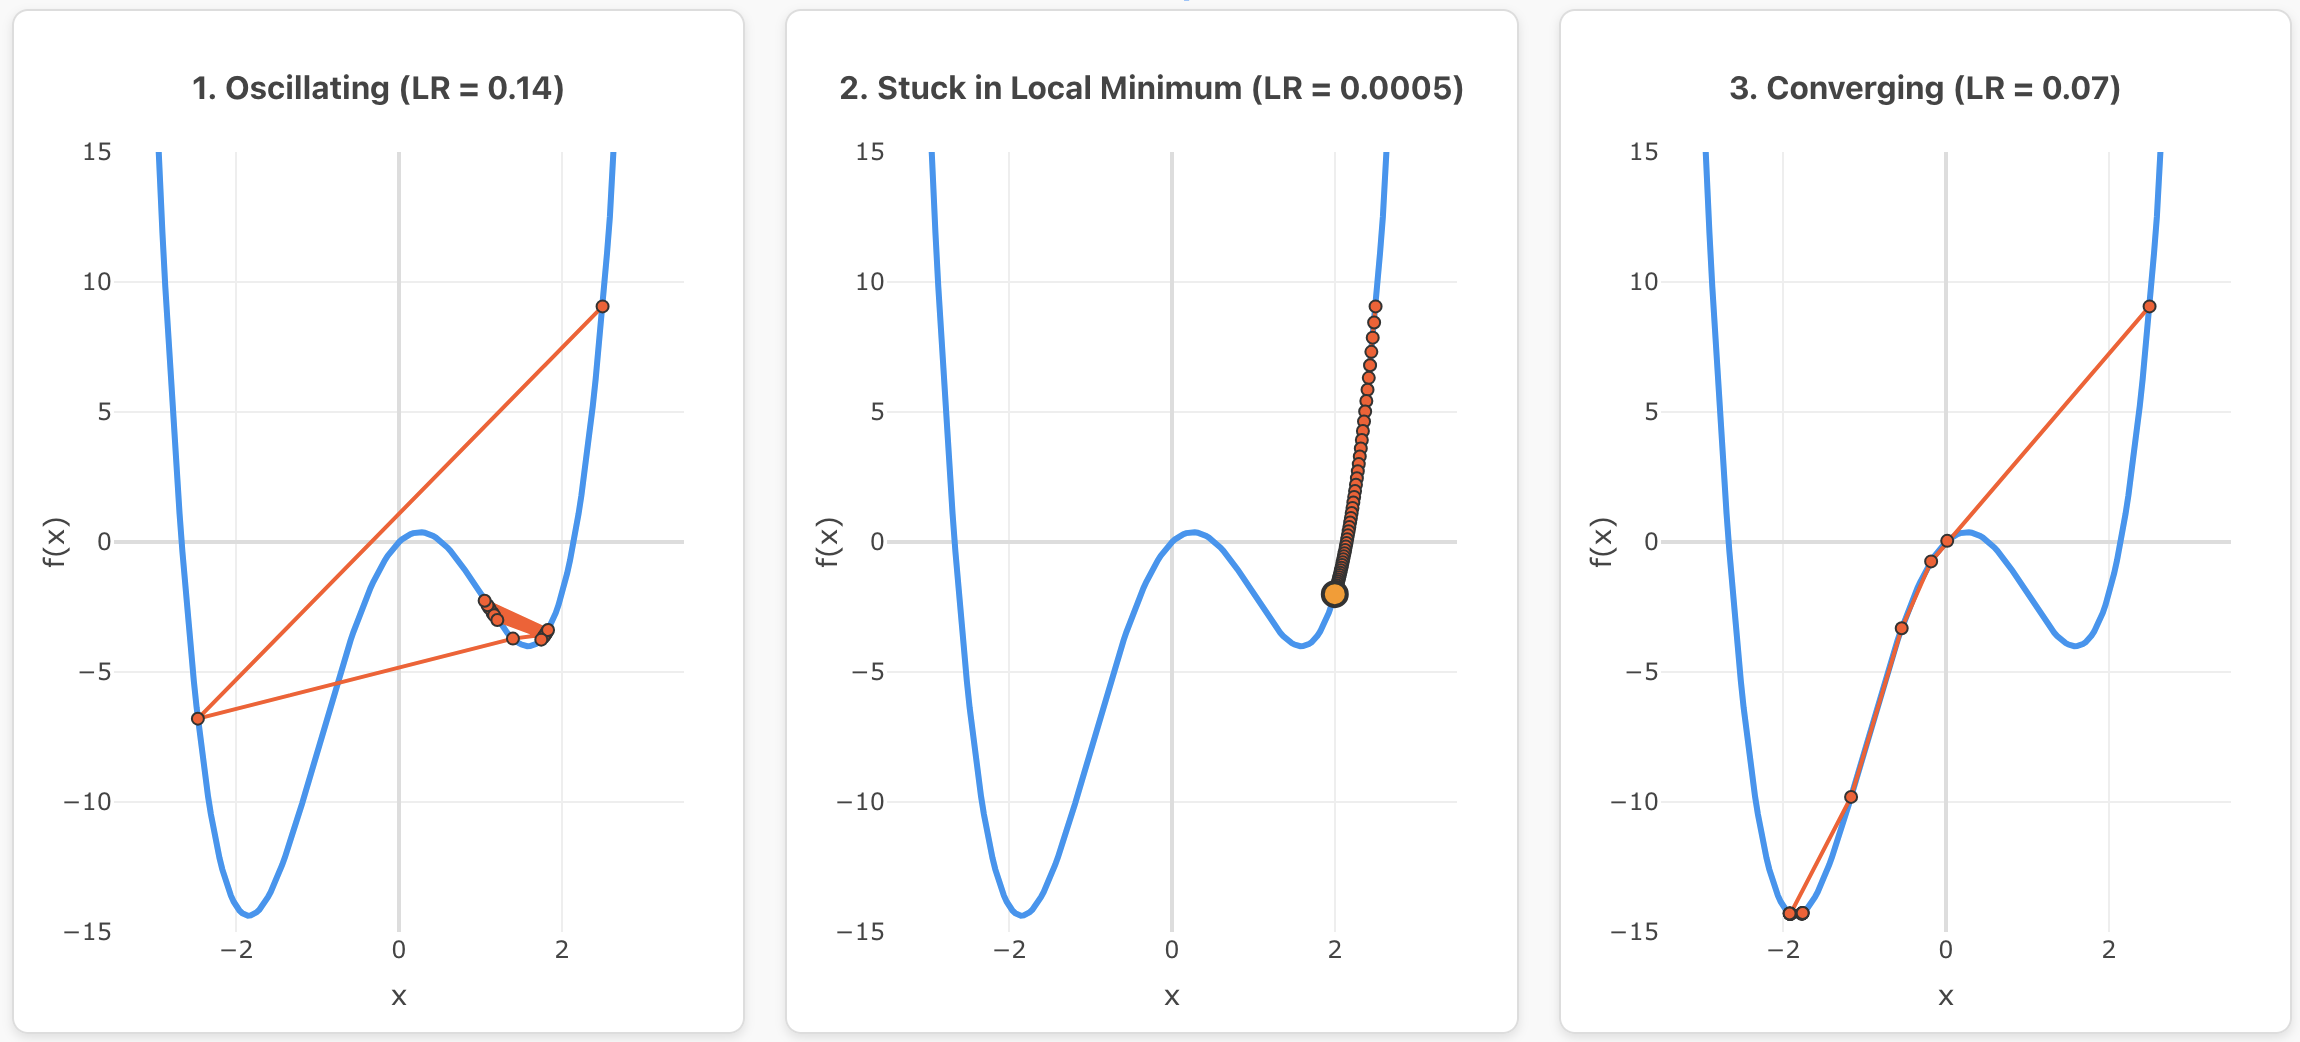
\includegraphics[width=0.8\textwidth]{sgd.gif}
\end{figure}

\begin{itemize}
    \item Too high: Overshooting, divergence
    \item Too low: Slow convergence, local minima
    \item Just right: Stable, efficient convergence
\end{itemize}
\end{frame}

%------------------------------------------------
\section{Overfitting and Regularization}
%------------------------------------------------

\begin{frame}
\frametitle{Overfitting}
\begin{figure}
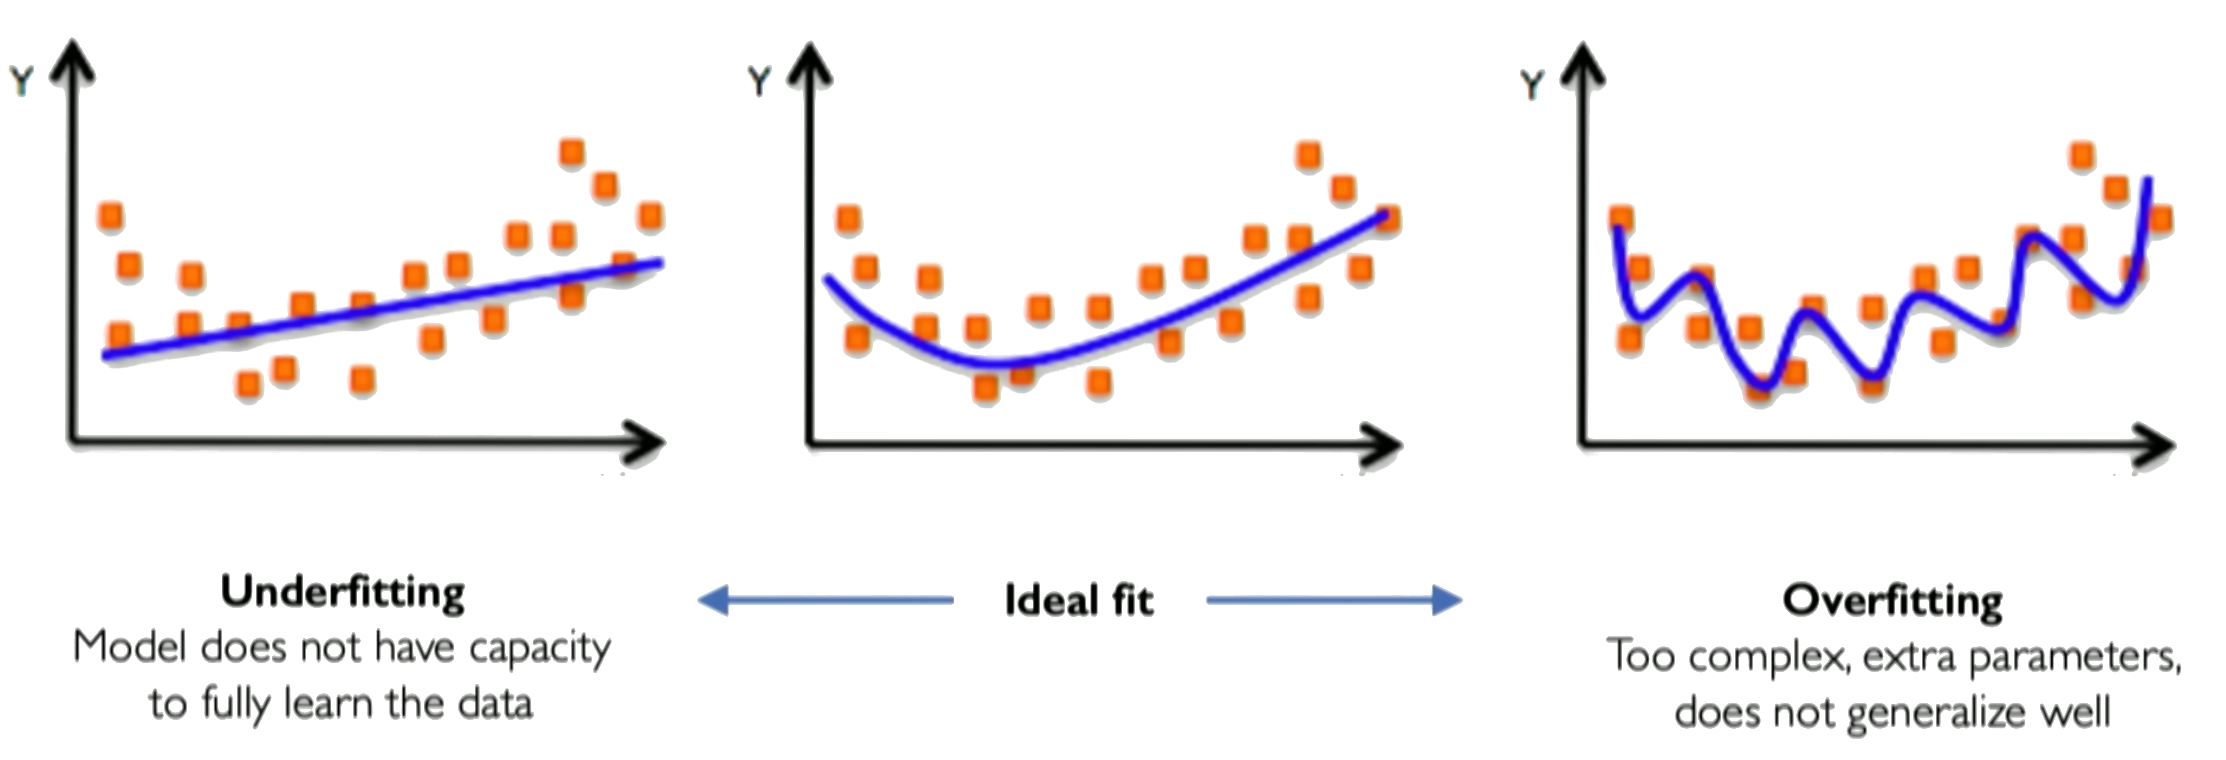
\includegraphics[width=0.8\textwidth]{overfitting.png}
\end{figure}

\begin{itemize}
    \item Model performs well on training data but poorly on new data
    \item Memorizes training examples instead of learning patterns
    \item Complex models are more prone to overfitting
\end{itemize}
\end{frame}

%------------------------------------------------
\begin{frame}
\frametitle{Training vs Validation Loss}
\begin{figure}
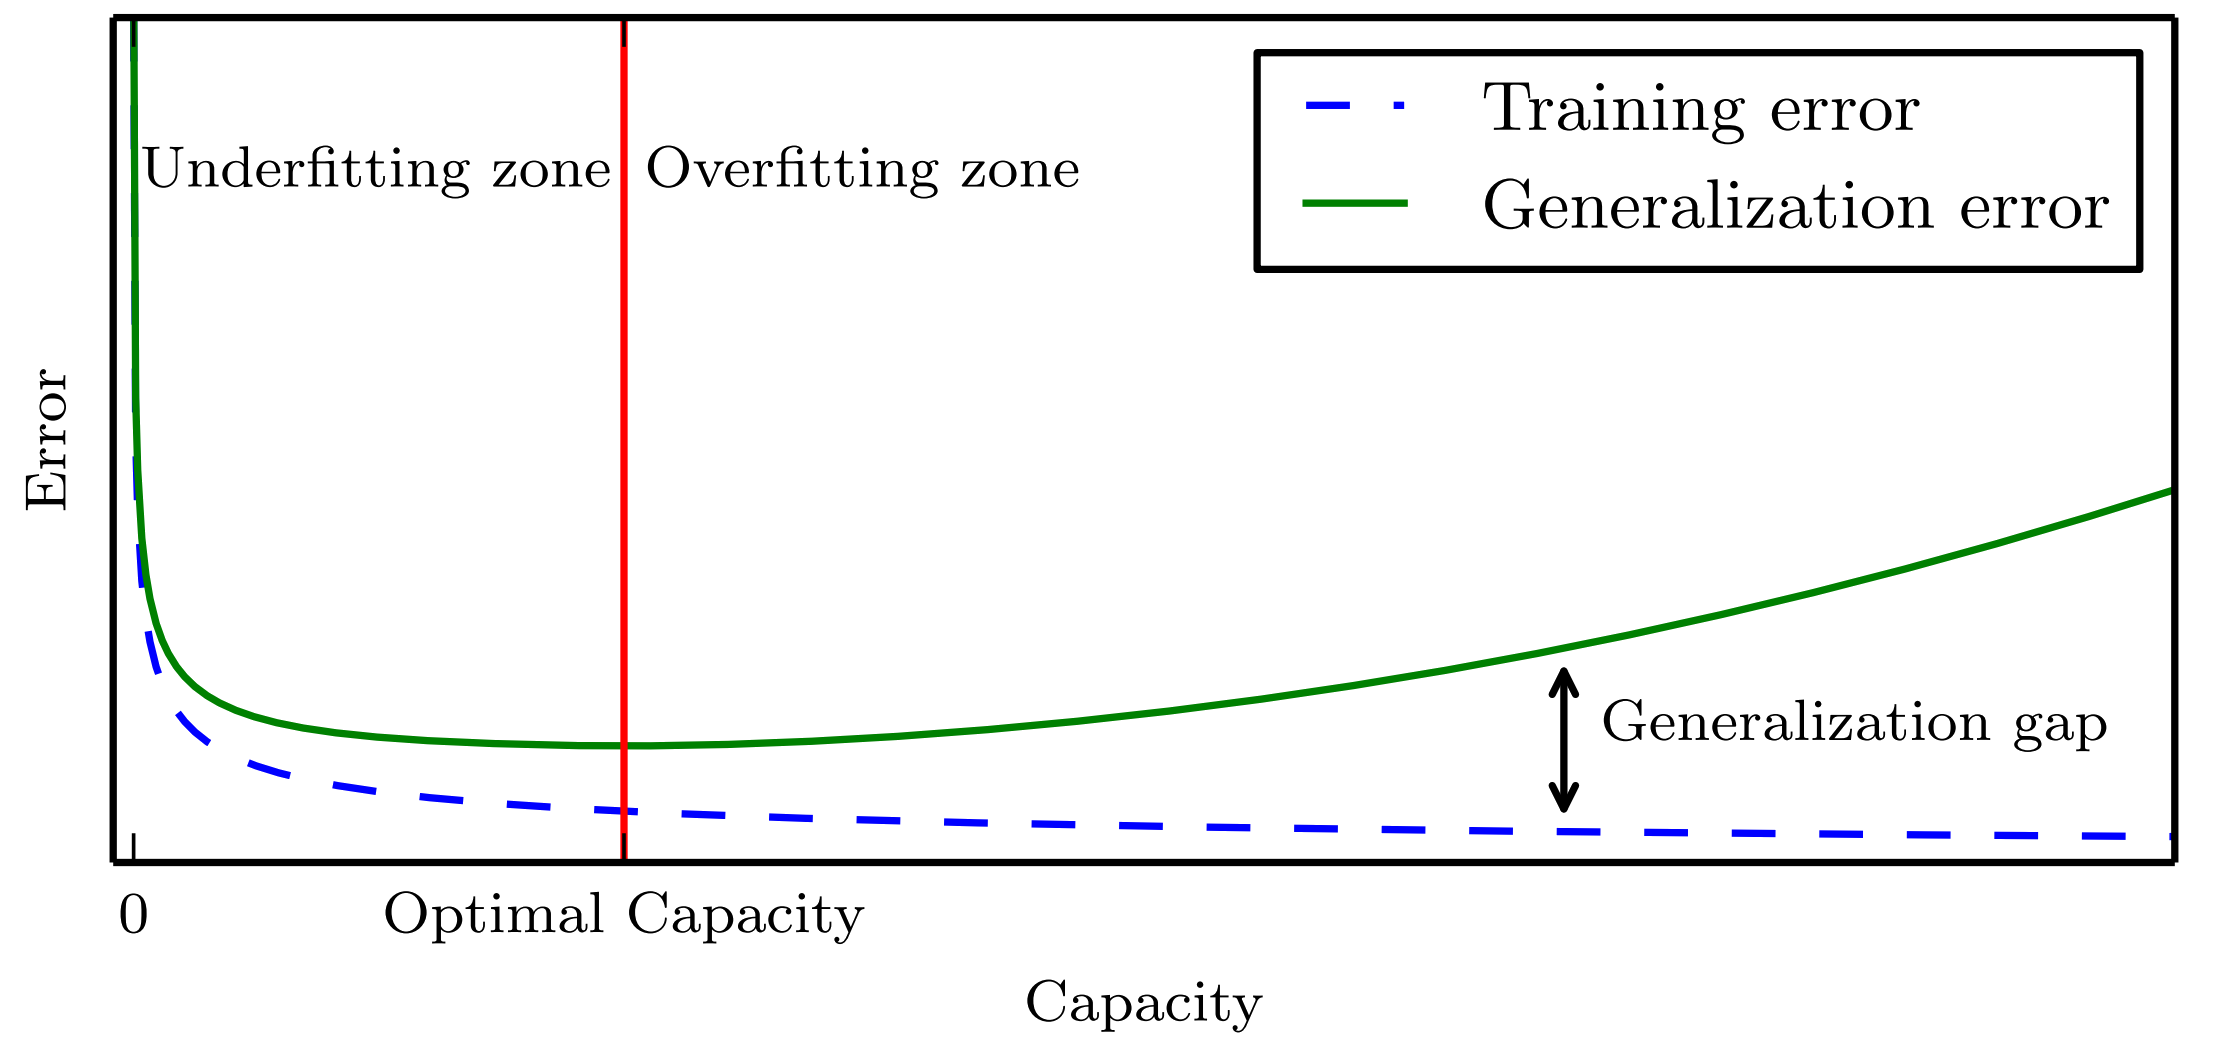
\includegraphics[width=0.8\textwidth]{training-validation-fit.png}
\end{figure}

\begin{itemize}
    \item \textbf{Underfitting:} High training and validation error
    \item \textbf{Good fit:} Low training and validation error
    \item \textbf{Overfitting:} Low training error, high validation error
\end{itemize}
\end{frame}

%------------------------------------------------
\begin{frame}
\frametitle{Regularization Techniques}
\textbf{Weight Decay (L2 Regularization):}
\begin{equation}
\mathcal{L}_{\text{reg}}(\boldsymbol{w}) = \mathcal{L}(\boldsymbol{w}) + \frac{\lambda}{2} |\|\boldsymbol{w}\||^2
\end{equation}

\textbf{Early Stopping:}
\begin{itemize}
    \item Monitor validation loss during training
    \item Stop when validation loss starts increasing
    \item Prevents overfitting without changing architecture
\end{itemize}

\textbf{Dropout:}
\begin{itemize}
    \item Randomly set neurons to zero during training
    \item Prevents co-adaptation of neurons
    \item Improves generalization
\end{itemize}
\end{frame}

%------------------------------------------------
\section{Scientific Machine Learning Applications}
%------------------------------------------------

\subsection{Constitutive Modeling}
%------------------------------------------------
\begin{frame}
\frametitle{Bingham Plastic Model}
\begin{figure}
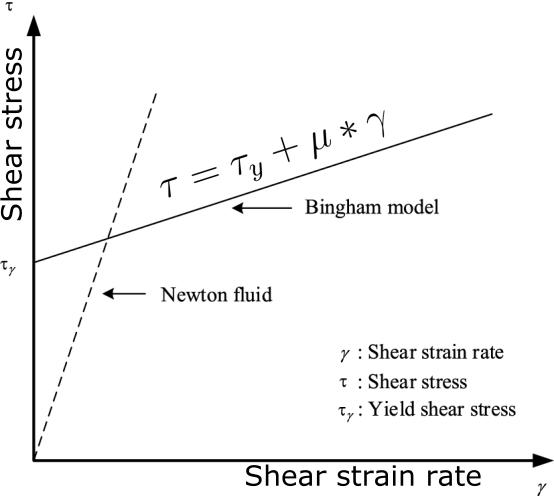
\includegraphics[width=0.6\textwidth]{bingham.png}
\end{figure}

\textbf{Traditional Model:}
\begin{equation}
\tau = \tau_y + \mu\dot{\gamma}
\end{equation}

\textbf{Neural Network Approach:}
\begin{equation}
\tau = \text{MLP}(\dot{\gamma}, \tau_y, \mu)
\end{equation}
\end{frame}

%------------------------------------------------
\begin{frame}
\frametitle{Herschel-Bulkley Model}
\begin{figure}
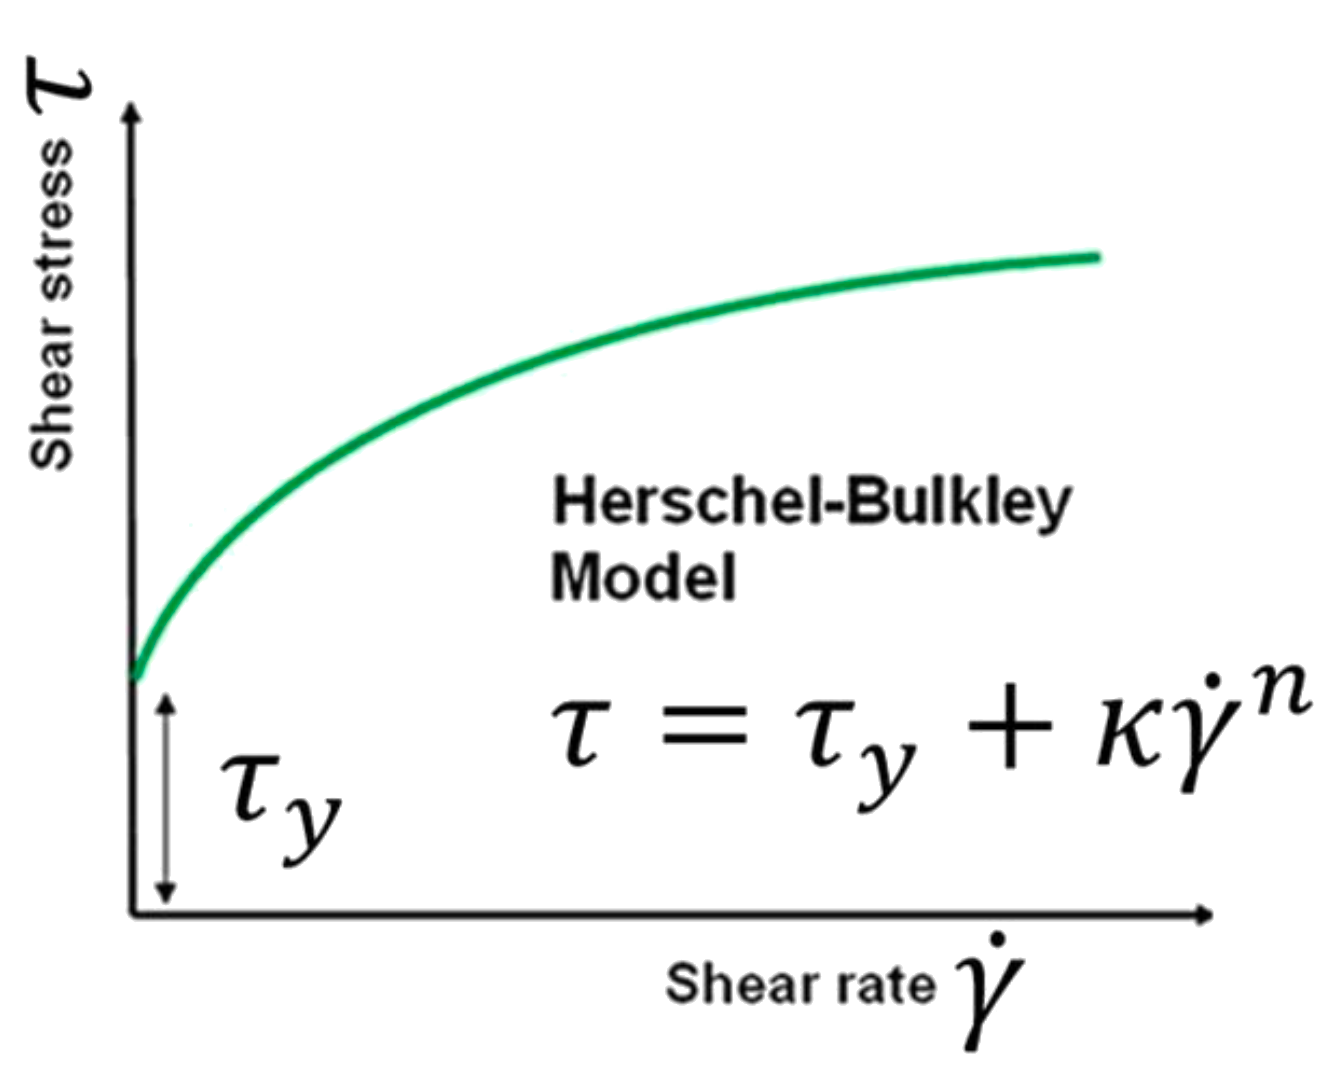
\includegraphics[width=0.6\textwidth]{herschel-bulkley.png}
\end{figure}

\textbf{Traditional Model:}
\begin{equation}
\tau = \tau_0 + k \dot{\gamma}^n
\end{equation}

\textbf{Neural Network Approach:}
\begin{equation}
\tau = \text{MLP}(\dot{\gamma}, \tau_0, k, n)
\end{equation}

More complex, non-linear behavior with multiple hidden layers.
\end{frame}

%------------------------------------------------
\section{Implementation}
%------------------------------------------------

\subsection{NumPy Implementation}
%------------------------------------------------
\begin{frame}[fragile]
\frametitle{NumPy MLP Implementation}
\begin{lstlisting}[language=Python, basicstyle=\tiny]
class NonLinearMLP_NumPy:
    def __init__(self, input_size, hidden_size, output_size):
        # Glorot Initialization
        limit_w1 = np.sqrt(6 / (input_size + hidden_size))
        self.W1 = np.random.uniform(-limit_w1, limit_w1, 
                                   (input_size, hidden_size))
        self.b1 = np.zeros((1, hidden_size))
        
        limit_w2 = np.sqrt(6 / (hidden_size + output_size))
        self.W2 = np.random.uniform(-limit_w2, limit_w2, 
                                   (hidden_size, output_size))
        self.b2 = np.zeros((1, output_size))

    def forward(self, x):
        self.z1 = np.dot(x, self.W1) + self.b1
        self.a1 = np.tanh(self.z1)
        y_pred = np.dot(self.a1, self.W2) + self.b2
        return y_pred
\end{lstlisting}
\end{frame}

%------------------------------------------------
\begin{frame}[fragile]
\frametitle{Training Loop}
\begin{lstlisting}[language=Python, basicstyle=\tiny]
def train_model_manual_sgd(model, x_data, y_data, epochs=50000, lr=0.1):
    n_samples = len(y_data)
    
    for epoch in range(epochs):
        y_pred = model.forward(x_data)
        loss = np.mean((y_pred - y_data)**2)
        
        # Backpropagation
        grad_y_pred = 2 * (y_pred - y_data) / n_samples
        grad_W2 = np.dot(model.a1.T, grad_y_pred)
        grad_b2 = np.sum(grad_y_pred, axis=0, keepdims=True)
        grad_a1 = np.dot(grad_y_pred, model.W2.T)
        grad_z1 = grad_a1 * (1 - np.tanh(model.z1)**2)
        grad_W1 = np.dot(model.x.T, grad_z1)
        grad_b1 = np.sum(grad_z1, axis=0, keepdims=True)
        
        # Parameter updates
        model.W1 -= lr * grad_W1
        model.b1 -= lr * grad_b1
        model.W2 -= lr * grad_W2
        model.b2 -= lr * grad_b2
\end{lstlisting}
\end{frame}

%------------------------------------------------
\subsection{PyTorch Implementation}
%------------------------------------------------
\begin{frame}[fragile]
\frametitle{PyTorch MLP Implementation}
\begin{lstlisting}[language=Python, basicstyle=\small]
import torch
import torch.nn as nn

class MLP(nn.Module):
    def __init__(self, input_size, hidden_size, output_size):
        super(MLP, self).__init__()
        self.hidden = nn.Linear(input_size, hidden_size)
        self.activation = nn.Tanh()
        self.output = nn.Linear(hidden_size, output_size)

    def forward(self, x):
        x = self.hidden(x)
        x = self.activation(x)
        x = self.output(x)
        return x

# Training
model = MLP(input_size=1, hidden_size=32, output_size=1)
criterion = nn.MSELoss()
optimizer = torch.optim.SGD(model.parameters(), lr=0.1)
\end{lstlisting}
\end{frame}

%------------------------------------------------
\section{Hyperparameter Tuning}
%------------------------------------------------

\begin{frame}
\frametitle{Key Hyperparameters}
\begin{itemize}
    \item \textbf{Learning Rate ($\eta$):} Controls optimization step size
    \item \textbf{Batch Size:} Affects gradient estimate and memory usage
    \item \textbf{Architecture:} Number of layers and neurons per layer
    \item \textbf{Activation Functions:} Affects gradient flow and expressiveness
    \item \textbf{Regularization:} Weight decay, dropout rate
    \item \textbf{Initialization:} Xavier, He, uniform, normal
    \item \textbf{Optimizer:} SGD, Adam, RMSprop
\end{itemize}

\vspace{1em}

\textbf{Hyperparameter Search:}
\begin{itemize}
    \item Grid search
    \item Random search
    \item Bayesian optimization
    \item Cross-validation
\end{itemize}
\end{frame}

%------------------------------------------------
\section{Common Challenges}
%------------------------------------------------

\begin{frame}
\frametitle{Common Challenges and Solutions}
\begin{table}[h]
\centering
\begin{tabular}{|l|l|}
\hline
\textbf{Challenge} & \textbf{Solutions} \\
\hline
Vanishing Gradients & ReLU, proper initialization, batch norm \\
\hline
Exploding Gradients & Gradient clipping, proper initialization \\
\hline
Overfitting & Regularization, dropout, early stopping \\
\hline
Underfitting & Increase model complexity, reduce regularization \\
\hline
Slow Convergence & Better optimizers (Adam), learning rate scheduling \\
\hline
Dead Neurons & Leaky ReLU, proper initialization \\
\hline
\end{tabular}
\end{table}

\vspace{1em}

\textbf{Best Practices:}
\begin{itemize}
    \item Start simple, then increase complexity
    \item Monitor training and validation metrics
    \item Use appropriate data preprocessing
    \item Regular checkpointing
\end{itemize}
\end{frame}

%------------------------------------------------
\section{Conclusion}
%------------------------------------------------

\begin{frame}
\frametitle{MLP Summary}
\textbf{Key Takeaways:}
\begin{itemize}
    \item MLPs are universal function approximators
    \item Hidden layers enable non-linear mappings
    \item Activation functions are crucial for expressiveness
    \item Backpropagation enables efficient gradient computation
    \item Regularization prevents overfitting
    \item Hyperparameter tuning is essential for performance
\end{itemize}

\vspace{1em}

\textbf{Applications in SciML:}
\begin{itemize}
    \item Constitutive modeling
    \item Surrogate modeling
    \item Parameter estimation
    \item Physics-informed neural networks (PINNs)
    \item Operator learning
\end{itemize}
\end{frame}

%------------------------------------------------
\begin{frame}
\frametitle{Next Steps}
\textbf{Advanced Topics:}
\begin{itemize}
    \item Convolutional Neural Networks (CNNs)
    \item Recurrent Neural Networks (RNNs)
    \item Physics-Informed Neural Networks (PINNs)
    \item Neural Operators
    \item Graph Neural Networks
    \item Transformers for Scientific Computing
\end{itemize}

\vspace{1em}

\textbf{Resources:}
\begin{itemize}
    \item Deep Learning (Goodfellow, Bengio, Courville)
    \item Neural Networks and Learning Machines (Haykin)
    \item Papers on Physics-Informed Neural Networks
    \item PyTorch and TensorFlow tutorials
\end{itemize}
\end{frame}

%------------------------------------------------
\begin{frame}
\frametitle{Questions?}
\begin{center}
\Huge Thank you!
\end{center}

\vspace{2em}

\begin{center}
\textbf{Contact:}\\
Krishna Kumar\\
\texttt{krishnak@utexas.edu}\\
\end{center}
\end{frame}

\end{document}
